\subsubsectionwithauthor[author={Mika Landeck},email={mika.landeck@fau.de}]{Aufgabe 1: Reguläre Sprachen}

\paragraph{(a)}m
		 
	$DEA = (\{ 1,2,3,4\},\{ a,b,c\},\delta,1,\{ 1,2\})$, wobei $\delta$ gegeben ist durch:
		
	\begin{tabular}{c|ccc}
		Zustand & a & b & c \\
		\hline
		1       & 2 & 1 & 1 \\
		2       & 3 & 1 & 1 \\
		3       & 4 & 1 & 4 \\
		4       & 4 & 4 & 4 \\
	\end{tabular} 
		
	Grafische Darstellung:
	\begin{center}
		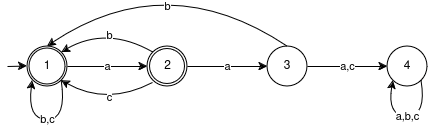
\includegraphics[scale=0.9]{DEA.png}
	\end{center}	
			
\paragraph{(b)}m
	Die Anzahl der Äquivalenzklassen kann die Anzahl an Zuständen nicht überschreiten, die der DEA aufweist, welcher diese Sprache erkennt. Der DEA aus a) verfügt über vier Zustände, also hat $L_1$ maximal vier Äquivalenzklassen.

	Wir finden vier unterschiedliche Äquivalenzklassen zu den Repräsentanten $\varepsilon, a, aa$ und $aaa$:
	\begin{itemize}
		\item Da $\varepsilon \circ a \in L_1$, aber $a \circ a \notin L_1$ gilt $[\varepsilon]\nsim_{L_1}[a]$.
		\item Da $\varepsilon \circ a \in L_1$, aber $aa \circ a \notin L_1$ gilt $[\varepsilon]\nsim_{L_1}[aa]$.
		\item Da $\varepsilon \circ a \in L_1$, aber $aaa \circ a \notin L_1$ gilt $[\varepsilon]\nsim_{L_1}[aaa]$.
		\item Da $a \circ c \in L_1$, aber $aa \circ c \notin L_1$ gilt $[a]\nsim_{L_1}[aa]$.
		\item Da $a \circ c \in L_1$, aber $aaa \circ c \notin L_1$ gilt $[a]\nsim_{L_1}[aaa]$.
		\item Da $aa \circ b \in L_1$, aber $aaa \circ b \notin L_1$ gilt $[aa]\nsim_{L_1}[aaa]$.
	\end{itemize}
	
	Drei Wörter je Äquivalenzklasse:
	\begin{enumerate}
		\item $bc, ccc, bbb \in [\varepsilon]$
		\item $a, aca, aba \in [a]$
		\item $aa, aabaa, abaa \in [aa]$
		\item $aaa, aac, aaabc \in [aaa]$
	\end{enumerate}
	\vspace{0.3cm}
	
	%\newpage
\paragraph{(c)}m 
	\textbf{Übergangstabelle}
	
	\begin{tabular}{|c|c|c|c|}
		\hline
		\textbf{Zustand}  & \textbf{a-Übergang} & \textbf{b-Übergang} & \textbf{$\epsilon$-Übergang} \\
		\hline
		1                 & 2                   & 1                   & 4 \\
		\hline
		2                 & 3                   & $\varnothing$       & $\varnothing$ \\
		\hline
		3                 & 1                   & 2                   & 1 \\
		\hline
		4                 & $\varnothing$       & 3                   & $\varnothing$ \\
		\hline
	\end{tabular}
	
	
	\textbf{$\epsilon$-Funktionsabschlusstabelle}
		
	\begin{tabular}{|c|c|}
		\hline
		\textbf{Zustand}  & \textbf{Funktionsabschluss} \\
		\hline
		1                 & \{1,4\} \\
		\hline
		2                 & \{2\} \\
		\hline
		3                 & \{1,3,4\}  \\
		\hline
		4                 & \{4\} \\
		\hline
	\end{tabular}
	
	\textbf{Pontenzmengenkonstruktionstabelle}
	
	\begin{tabular}{|c|c|c|c|}
		\hline
		\textbf{Zustand} & \textbf{a-Übergang} & \textbf{b-Übergang} & \textbf{Endzustand?} \\
		\hline
		\{1,4\}     & \{2\}       & \{1,3,4\}         & Ja \\
		\hline
		\{2\}       & \{1,3,4\}   & \{$\varnothing$\} &    \\
		\hline
		\{1,3,4\}   & \{1,2,4\}   & \{1,2,3,4\}       & Ja \\
		\hline
		\{1,2,4\}   & \{1,2,3,4\} & \{1,3,4\}         & Ja \\
		\hline
		\{1,2,3,4\} & \{1,2,3,4\} & \{1,2,3,4\}       & Ja \\
		\hline
		\{$\varnothing$\}       & \{$\varnothing$\}   & \{$\varnothing$\} &    \\
		\hline
	\end{tabular}	
	
	\textbf{Fertiger DEA} \\
	
	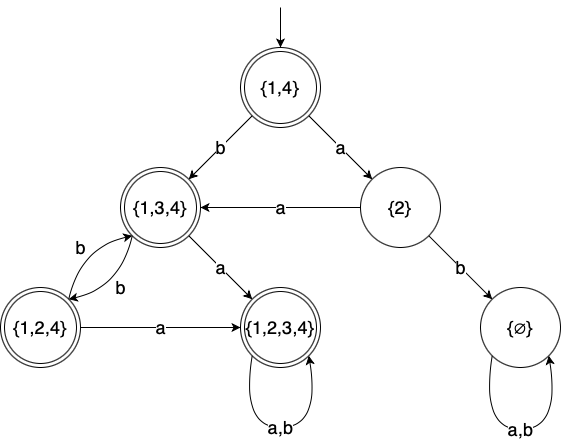
\includegraphics[scale=0.5]{NEA-DEA}
	


\newpage